\documentclass{beamer}

\usepackage[utf8]{inputenc}
\usepackage[ngerman]{babel}
\usepackage{amssymb}
\usepackage{amsmath}
\usepackage{graphicx}

\usetheme{Warsaw}

\title{Hochwasserstände vorhersagen mittels Kleinste-Quadrate-Lösung}
\author{Marisa Breßler und Anne Jeschke}
\date{21.01.2020}

\begin{document}
\setbeamertemplate{footline}
{%
\begin{beamercolorbox}[wd=0.5\textwidth,ht=3ex,dp=1.5ex,leftskip=.5em,rightskip=.5em]{author in head/foot}%
\usebeamerfont{author in head/foot}%
\insertframenumber\hfill\insertshortauthor%
\end{beamercolorbox}%
\vspace*{-4.5ex}\hspace*{0.5\textwidth}%
\begin{beamercolorbox}[wd=0.5\textwidth,ht=3ex,dp=1.5ex,left,leftskip=.5em]{title in head/foot}%
\usebeamerfont{title in head/foot}%
\insertshorttitle%
\end{beamercolorbox}%
}

\maketitle
\frame{\tableofcontents}

\section{Einleitung}
\begin{frame} %%Eine Folie
  \frametitle{Vorstellung des Problems} %%Folientitel

  \underline{Ziel}: in Daten Zusammenhang erkennen, um Prognosen zu erstellen

  \begin{table}
    \centering
    \tabcolsep=0.11cm
    \begin{tabular}{c|cccccccccccc}
      $p_0$ & 172 & 309 & 302 & 283 & 443 & 298 & 319 & 419 & 361 & 267 & 337 & 230 \\ \hline
      $p_1$ & 93 & 193 & 187 & 174 & 291 & 184 & 205 & 260 & 212 & 169 & 216 & 144 \\ \hline
      $p_2$ & 120 & 258 & 255 & 238 & 317 & 246 & 265 & 304 & 292 & 242 & 272 & 191
    \end{tabular}
  \caption{Pegelstände an den Stellen $p_0$, $p_1$ und $p_2$}
  \end{table}
\end{frame}

\section{Theorie}
\begin{frame} %%Eine Folie
  \frametitle{Aufstellung eines Gleichungssystems} %%Folientitel
  \tabcolsep=0.11cm
  \begin{table}
    \centering
  \begin{tabular}{c|cccccccccccc}
    $p_0$ & 172 & 309 & 302 & 283 & 443 & 298 & 319 & 419 & 361 & 267 & 337 & 230 \\ \hline
    $p_1$ & 93 & 193 & 187 & 174 & 291 & 184 & 205 & 260 & 212 & 169 & 216 & 144
  \end{tabular}
  \caption{Pegelstände an den Stellen $p_0$ und $p_1$}
\end{table}

\centering
$p_{0,i} = x_1 p_{1,i} + x_2 \thickspace \thickspace \forall i = 1,...,N$
\pause

\begin{equation*}
\begin{array}{cccccc}
&\begin{pmatrix}
  p_{0,1}\\
  p_{0,2}\\
  \vdots \\
  p_{0,N}
\end{pmatrix}
  &=&
\begin{pmatrix}
  p_{1,1} & 1\\
  p_{1,2} & 1\\
  \vdots & \vdots\\
  p_{1,N} & 1
 \end{pmatrix}
  &\cdot&
  \begin{pmatrix}
    x_1\\
    x_2
  \end{pmatrix}\\
  \\
  \iff&b &=& A &\cdot &x
\end{array}
\end{equation*}
\end{frame}

\begin{frame} %%Eine Folie
  \frametitle{Methode der kleinsten Quadrate} %%Folientitel
  \underline{Gesucht}: Lösungsvektor x von $Ax=b$, s.d. $||Ax-b||_2$ minimal
  \begin{figure}
    \centering
      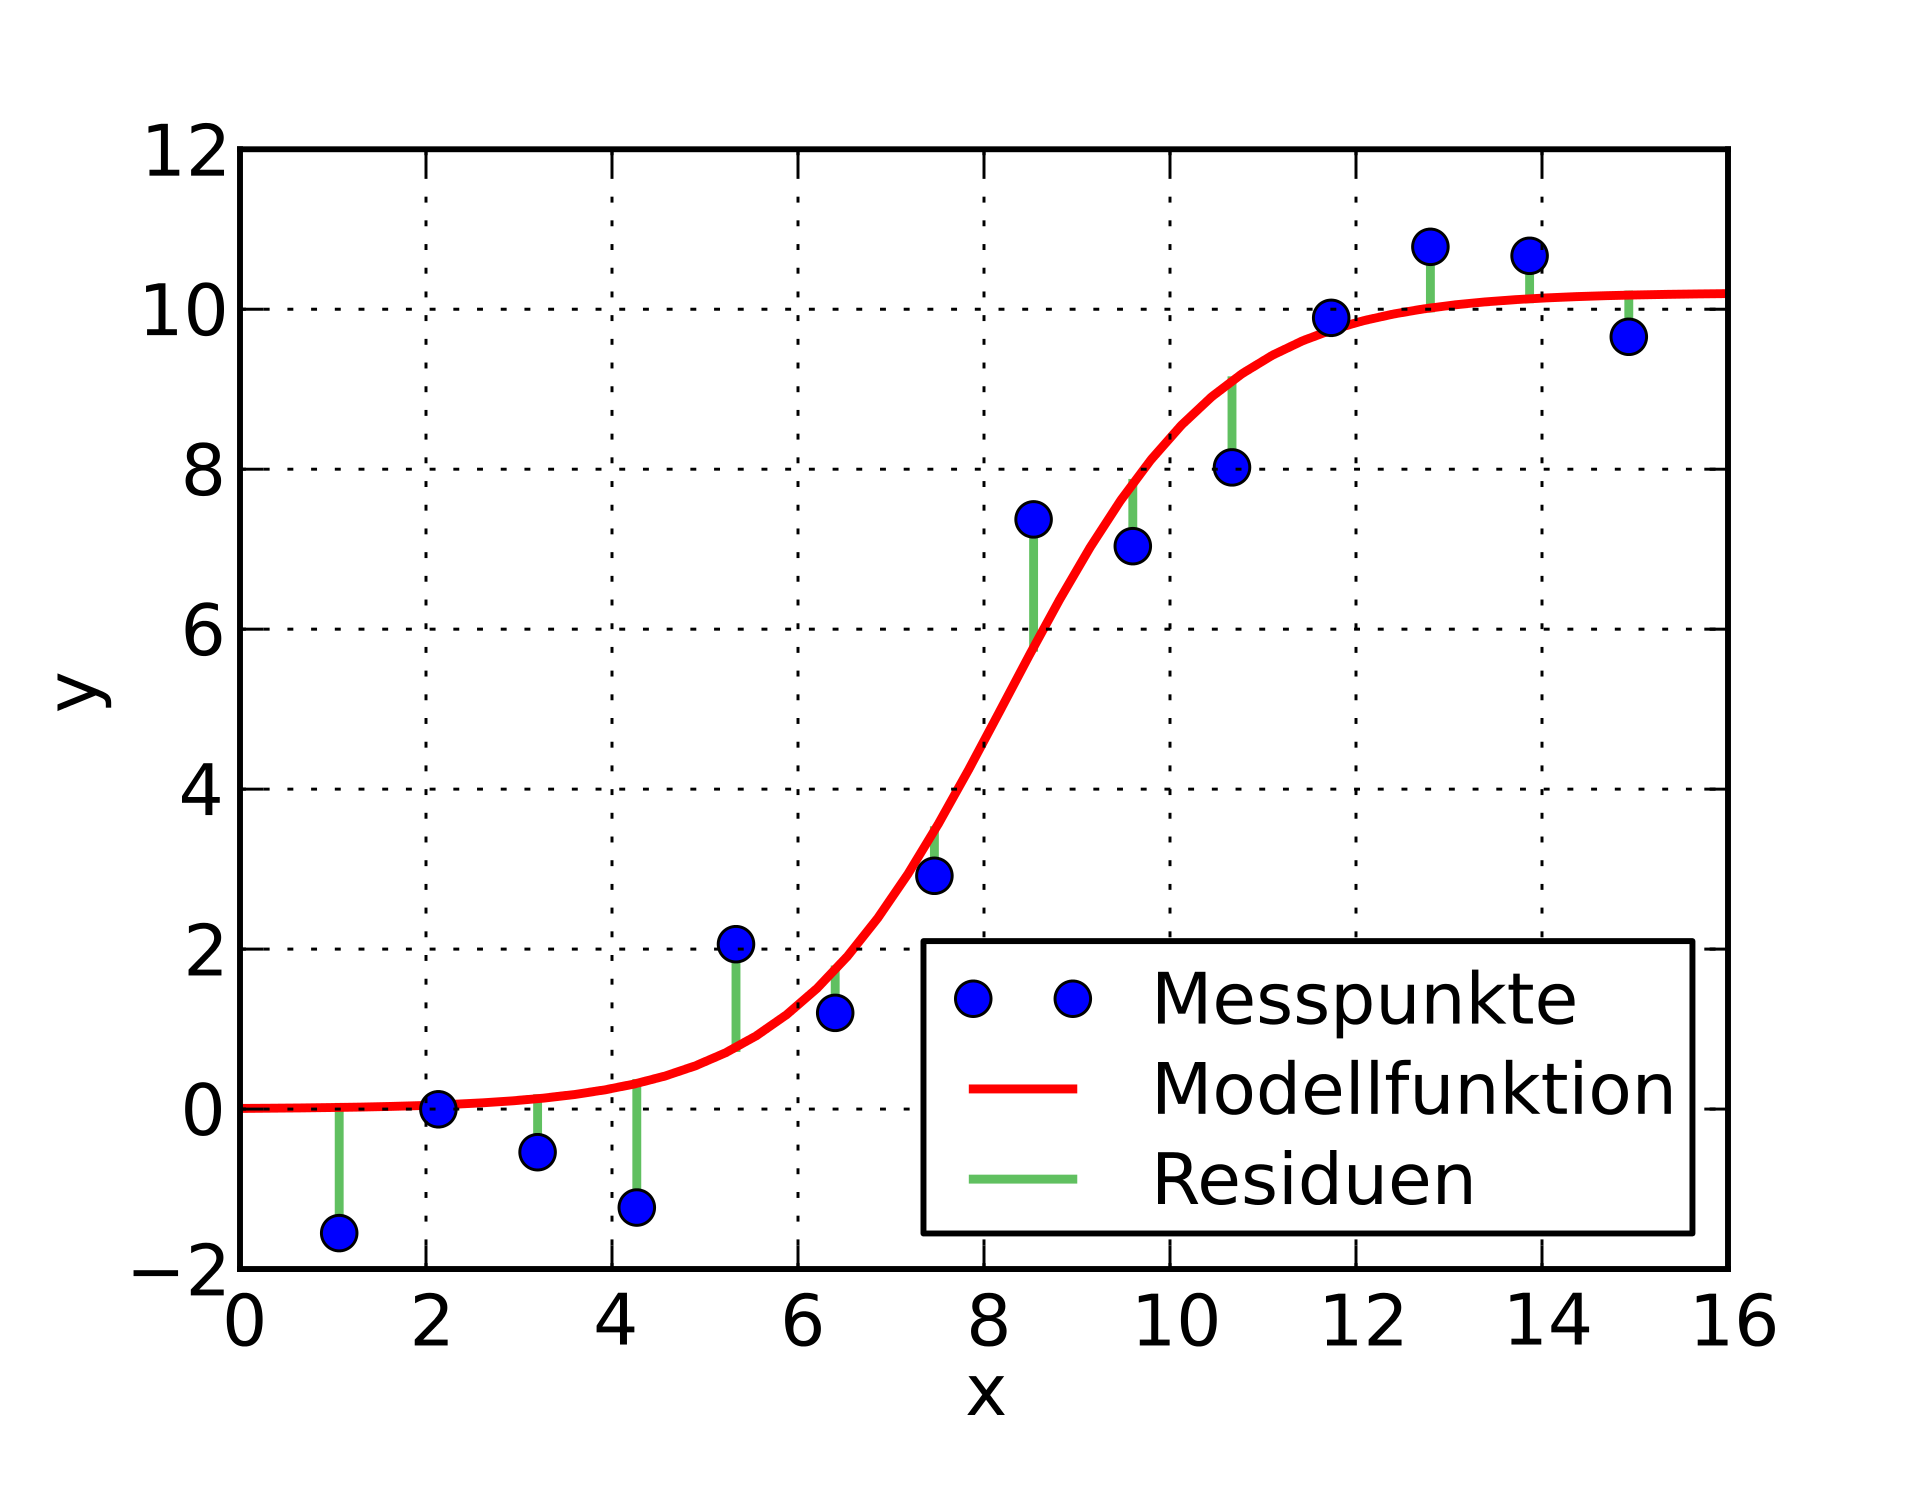
\includegraphics[width=0.6\textwidth]{least_squares_example}
    \caption{Beispiel einer Kleinste-Quadrate-Lösung, https://commons.wikimedia.org/w/index.php?curid=12879531}
  \end{figure}
\end{frame}

\begin{frame} %%Eine Folie
  \frametitle{Lösung mittels QR-Zerlegung} %%Folientitel
  \begin{equation*}
    Ax = b \iff QRx = b \iff Rx = Q^T b
  \end{equation*}
\bigskip

\centering
  $Q \in \mathbb{R}^{N\times N}$, orthogonal
\bigskip

  $R=
    \begin{pmatrix}
      R_1 \\
      R_2
    \end{pmatrix}$
  mit
  $R_1=
  \begin{pmatrix}
    *     & * \\
    0     & *\\
  \end{pmatrix} \in \mathbb{R}^{2\times 2}$
  und
  $R_2=0  \in \mathbb{R}^{(N-2)\times 2}$

\pause
\bigskip

  \begin{enumerate}
    \item $z := Q^T b$ mit
    $z =
    \begin{pmatrix}
      z_1 \\
      z_2
    \end{pmatrix}$
    , $z_1 \in \mathbb{R}^{2}$ und $z_2 \in \mathbb{R}^{N-2}$
    \pause
    \item Löse $R_1 x = z_1$ mittels Rückwärtseliminierung
    \pause
    \item $||Ax-b||_2 = ||z_2||_2$ ist minimal
  \end{enumerate}
\end{frame}

\section{Experimente}
\subsection{Einfache lineare Regression}

\begin{frame} %%Eine Folie
  \frametitle{Ergebnis mit unmodifizierten Daten} %%Folientitel
\begin{figure}
  \centering
    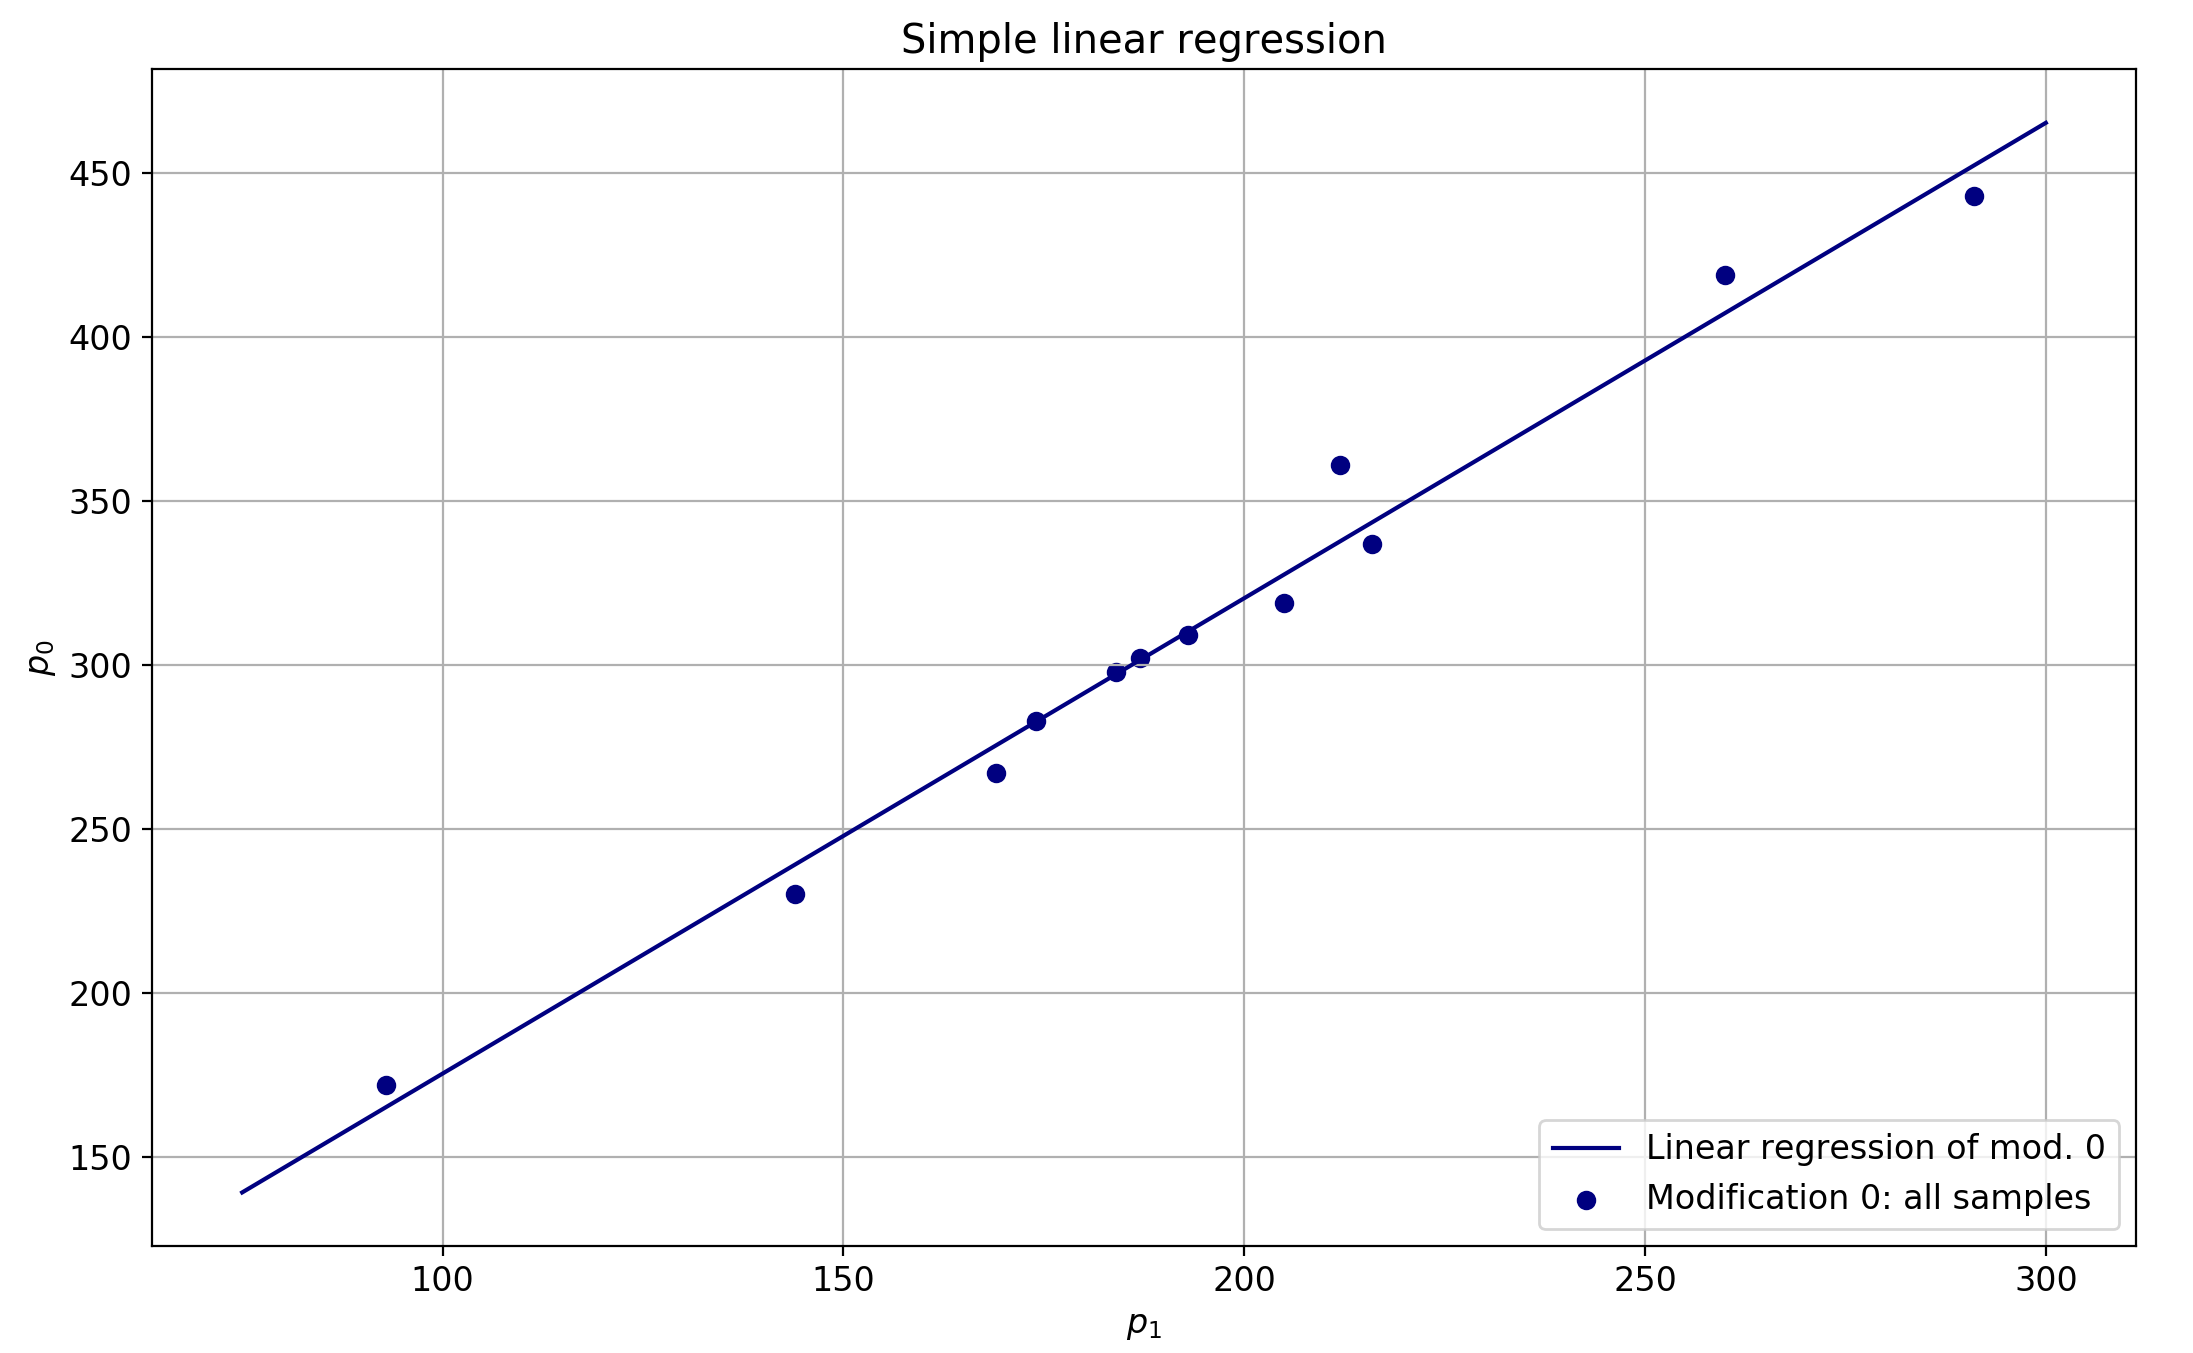
\includegraphics[width=0.75\textwidth]{unmodified}
    \vspace{-1em}
  \caption{Ergebnis mit unmodifizierten Daten}
\end{figure}
\vspace{-1em}
\centering
$p_0 = 1.450333p_1+30.302158$, $||Ax-b||_2=32.904232$

\end{frame}

\begin{frame} %%Eine Folie
  \frametitle{Ergebnisse mit modifizierten Daten} %%Folientitel
  \begin{figure}
    \centering
      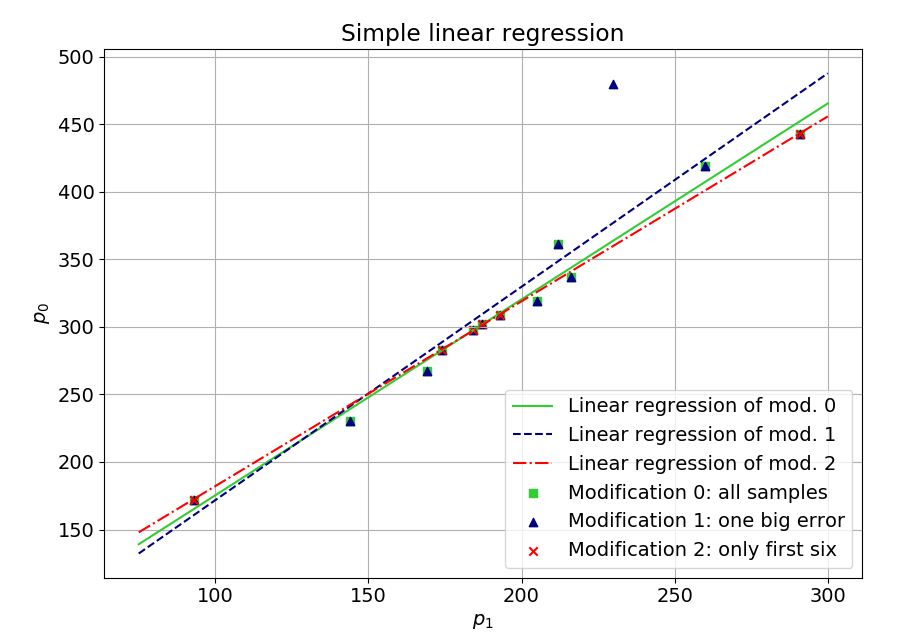
\includegraphics[width=0.9\textwidth]{Linear_Regression}
      \vspace{-1em}
    \caption{Ergebnis mit verschiedenen modifizierten Daten}
  \end{figure}
\end{frame}

\begin{frame}
  \begin{figure}
    \centering
      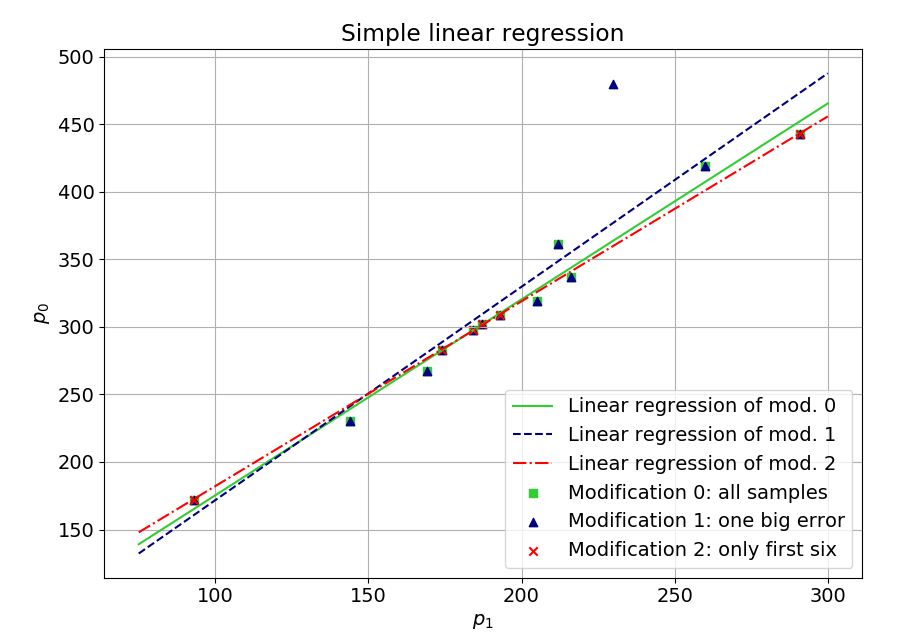
\includegraphics[width=0.8\textwidth]{Linear_Regression}
  \end{figure}
  \vspace{-1em}
  \centering
  \begin{tabular}{c|c|c}
    Nr. der Modifikation & $cond_2(A)$   & $||Ax-b||_2$\\ \hline
                       0 & $820.140820$  & $32.904232$\\ \hline
                       1 & $857.010517$  & $114.146281$\\ \hline
                       2 & $665.277296$  & $1.542414$
  \end{tabular}
\end{frame}

\begin{frame} %%Eine Folie
  \frametitle{Verwendung von anderer Messung} %%Folientitel
  \begin{figure}
    \centering
      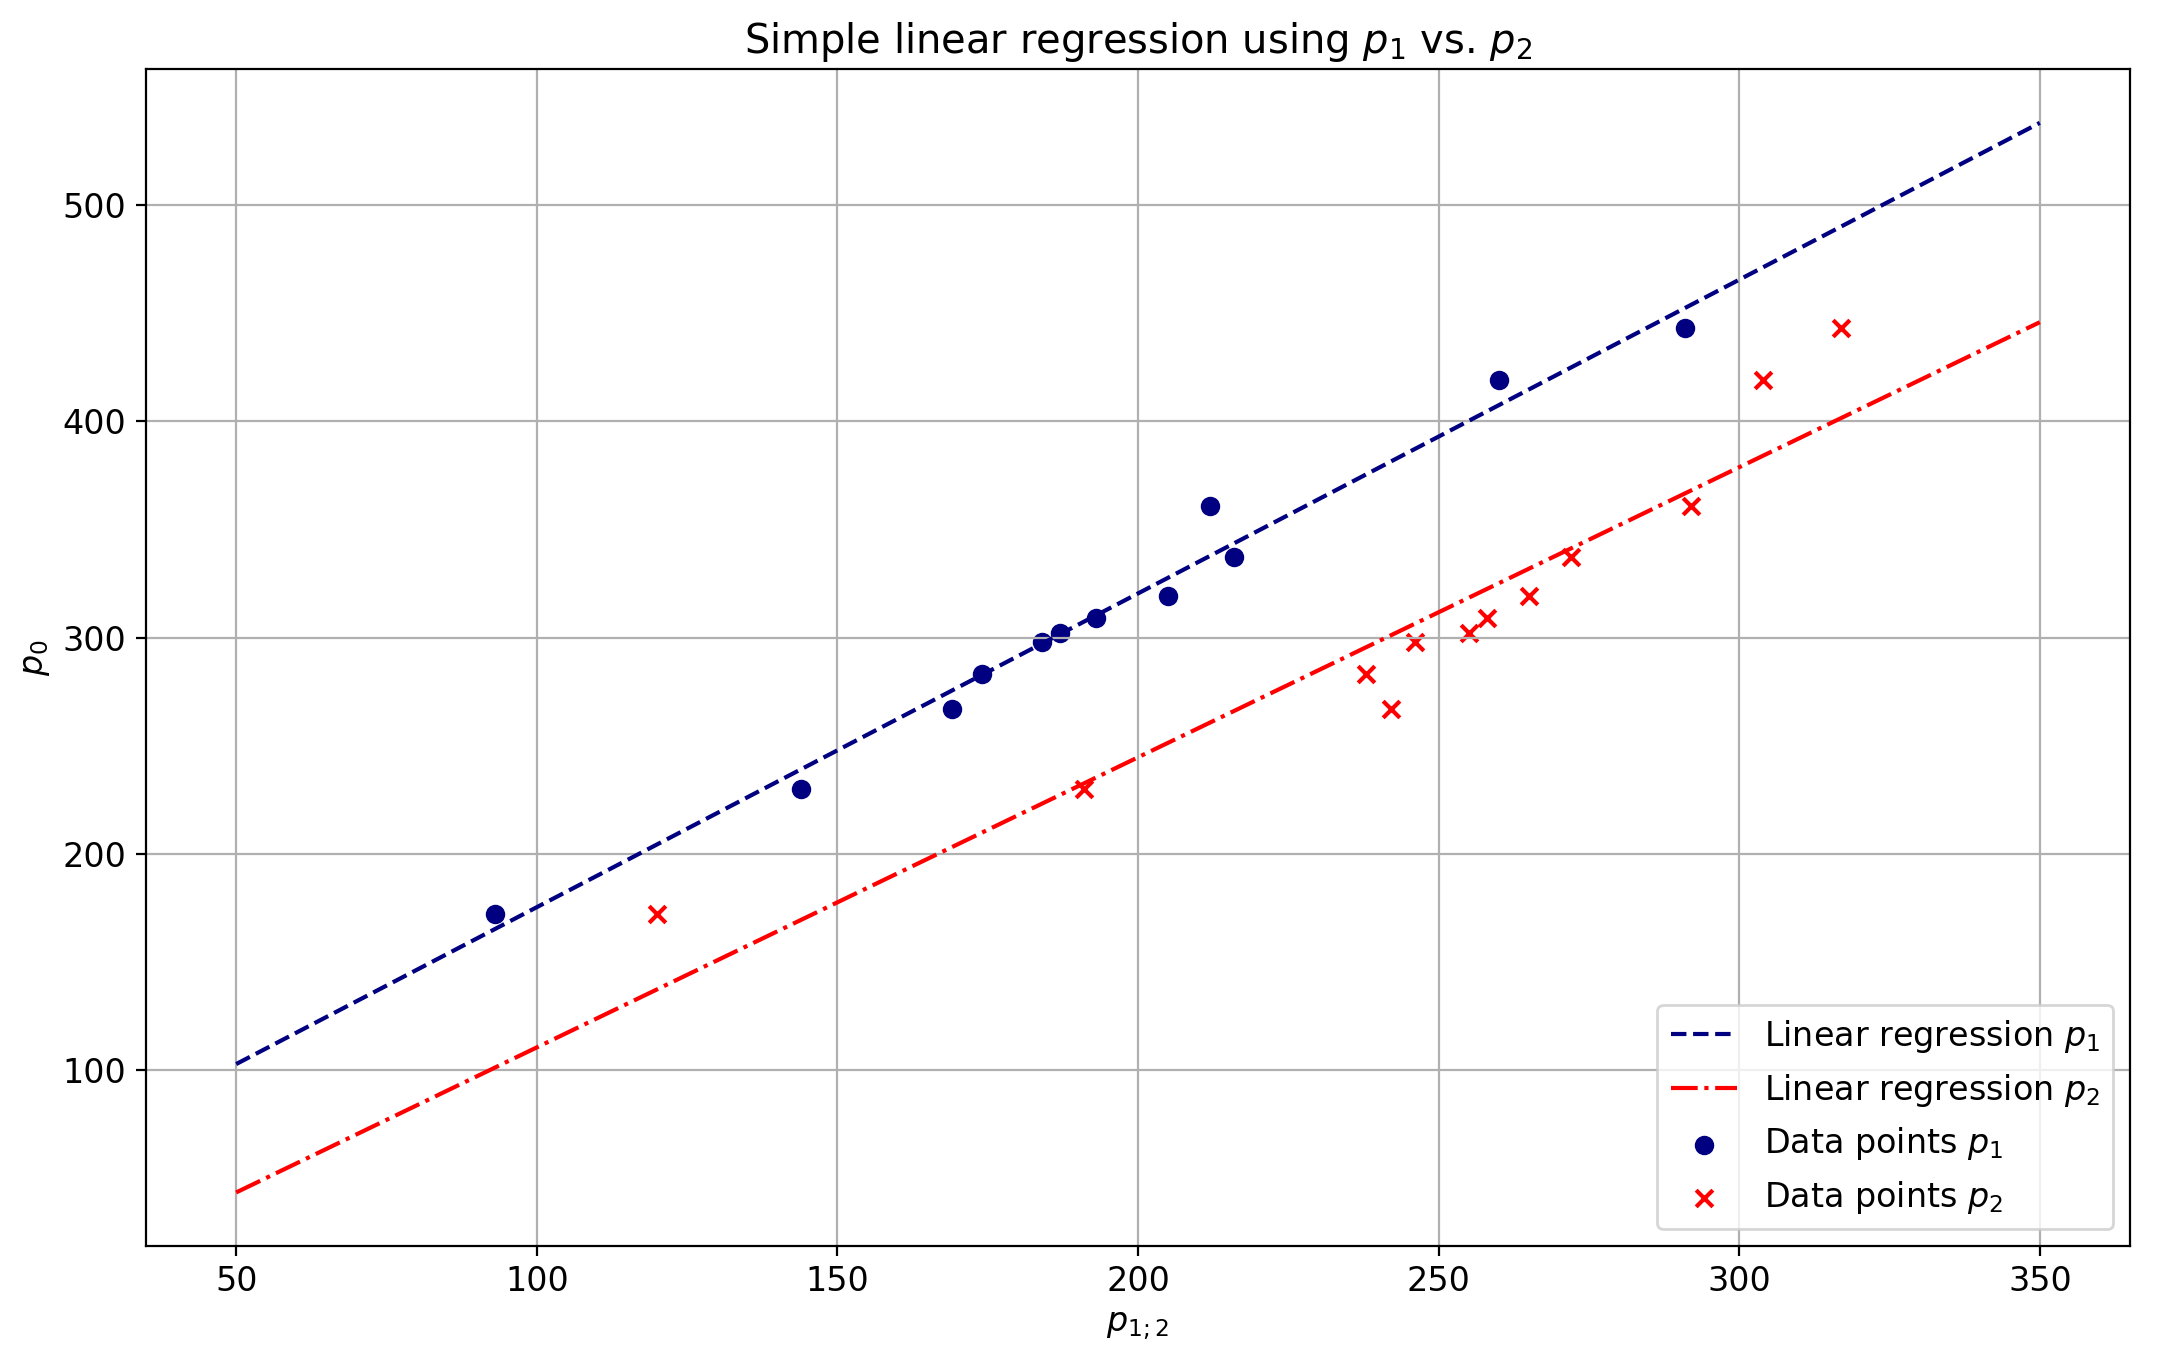
\includegraphics[width=0.9\textwidth]{Linear_Regression_p2}
      \vspace{-1em}
    \caption{Ergebnis mit $p_1$ vs. $p_2$}
  \end{figure}
\end{frame}
\begin{frame}
  \begin{figure}
    \centering
      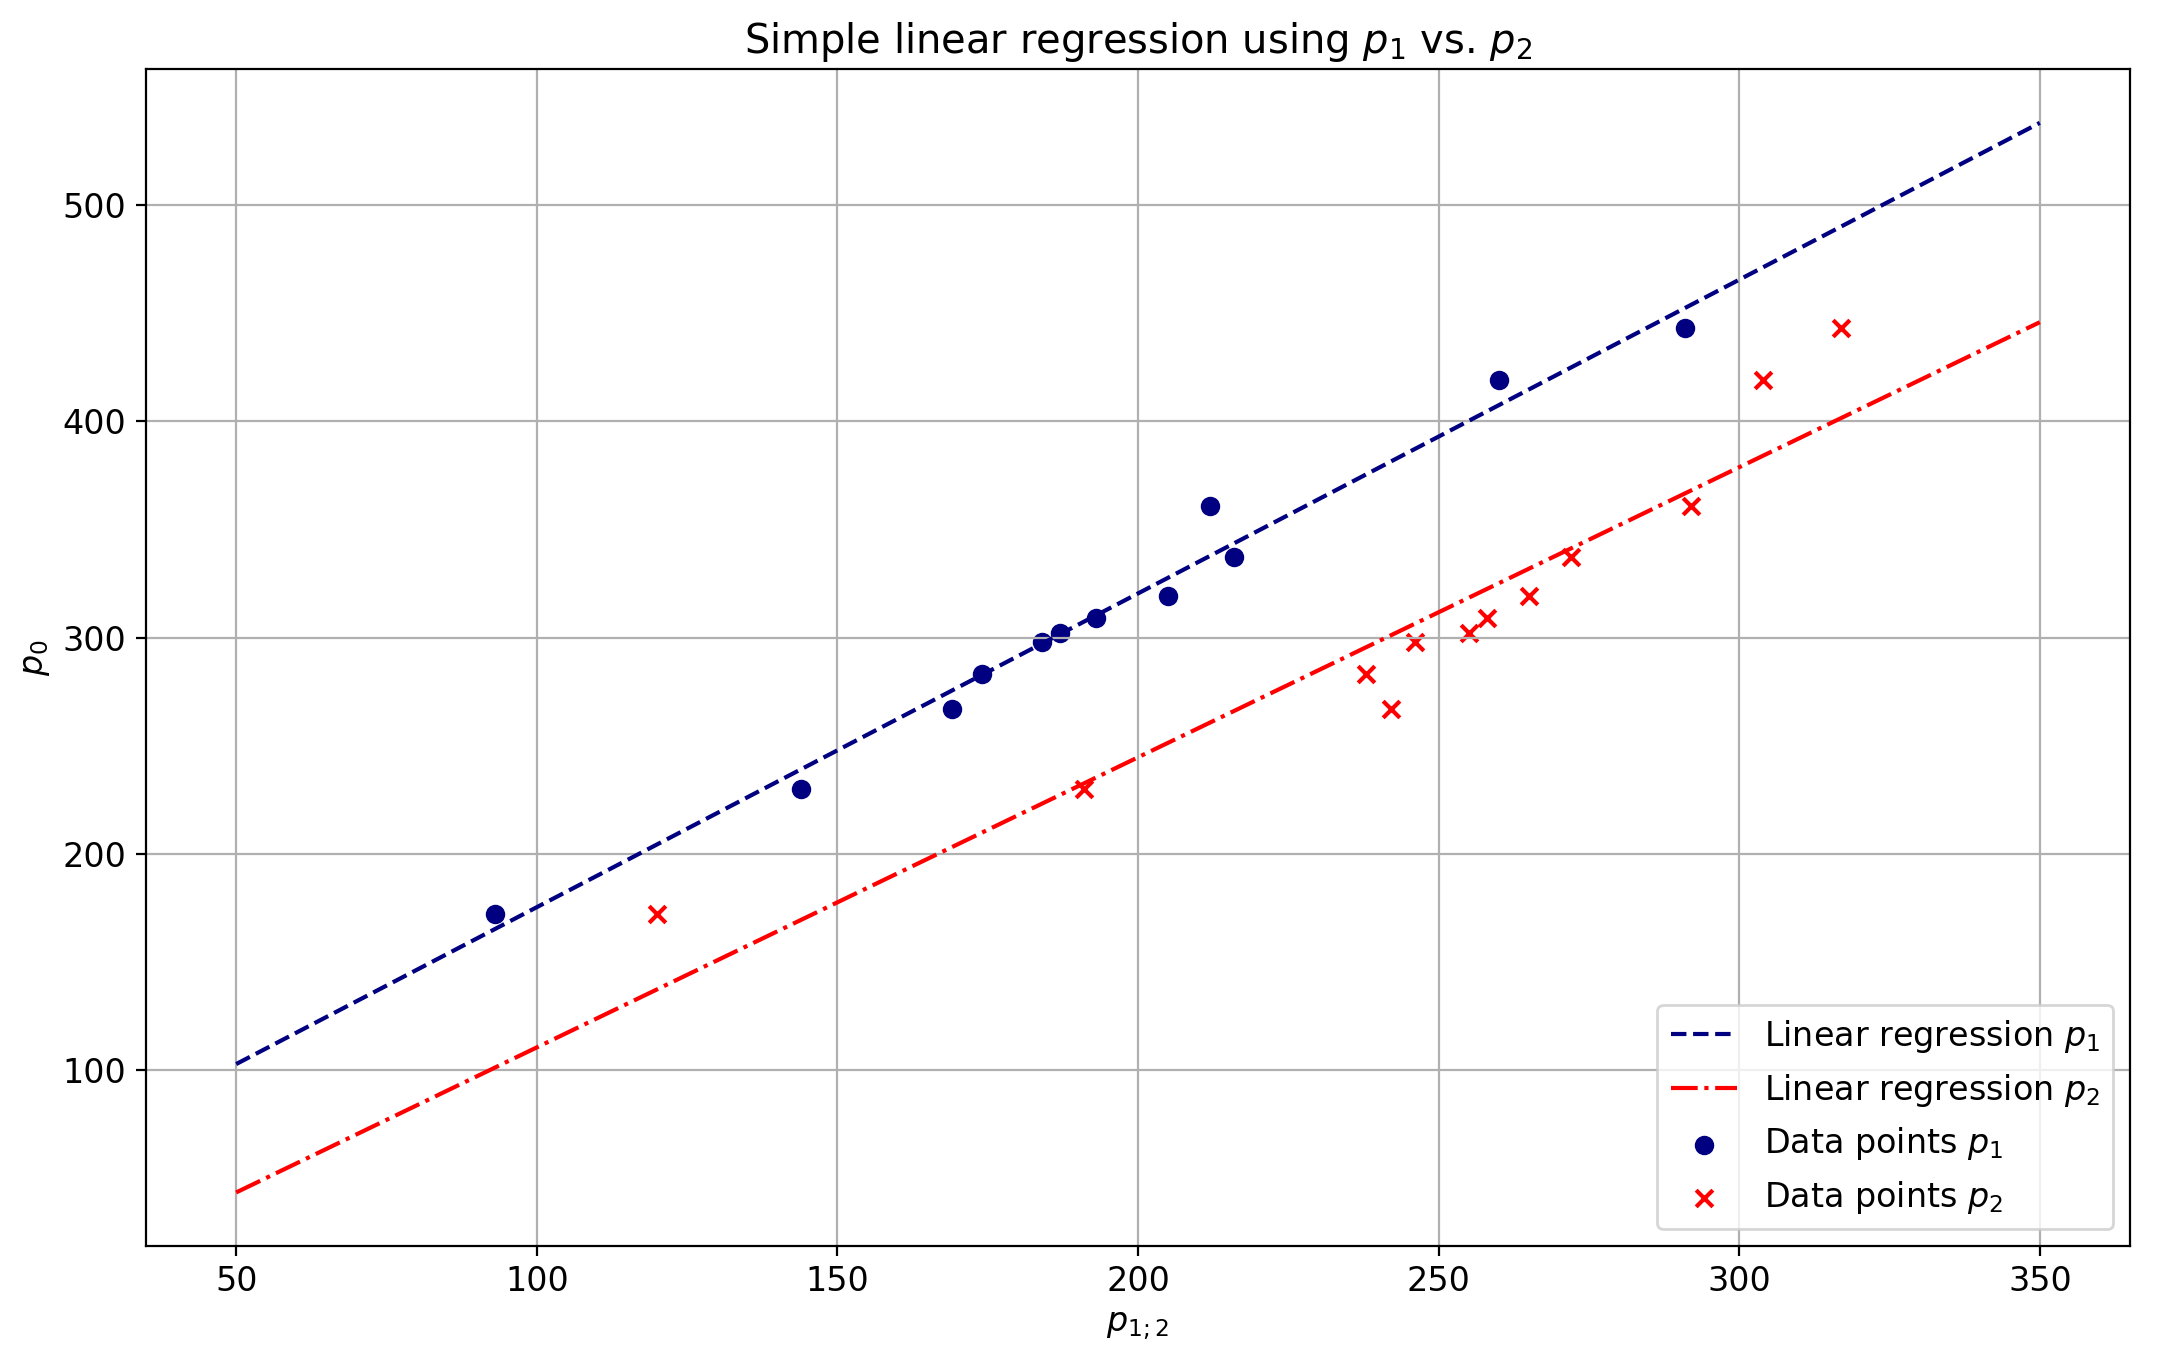
\includegraphics[width=0.8\textwidth]{Linear_Regression_p2}
  \end{figure}
  \vspace{-1em}
  \centering
  \begin{tabular}{c|c|c}
    Nr. des Pegels & $cond_2(A)$   & $||Ax-b||_2$\\ \hline
                 1 & $820.140820$  & $32.904232$\\ \hline
                 2 & $1288.744531$ & $78.768276$
  \end{tabular}
\end{frame}

\subsection{Lineare Mehrfachregression}
\begin{frame} %%Eine Folie
  \frametitle{Lineare Mehrfachregression} %%Folientitel
\centering
$p_{0,i} = x_1 p_{1,i} + x_2 p_{2, i} + x_3 \thickspace \thickspace \forall i = 1,...,N$

  \begin{figure}

    \centering
      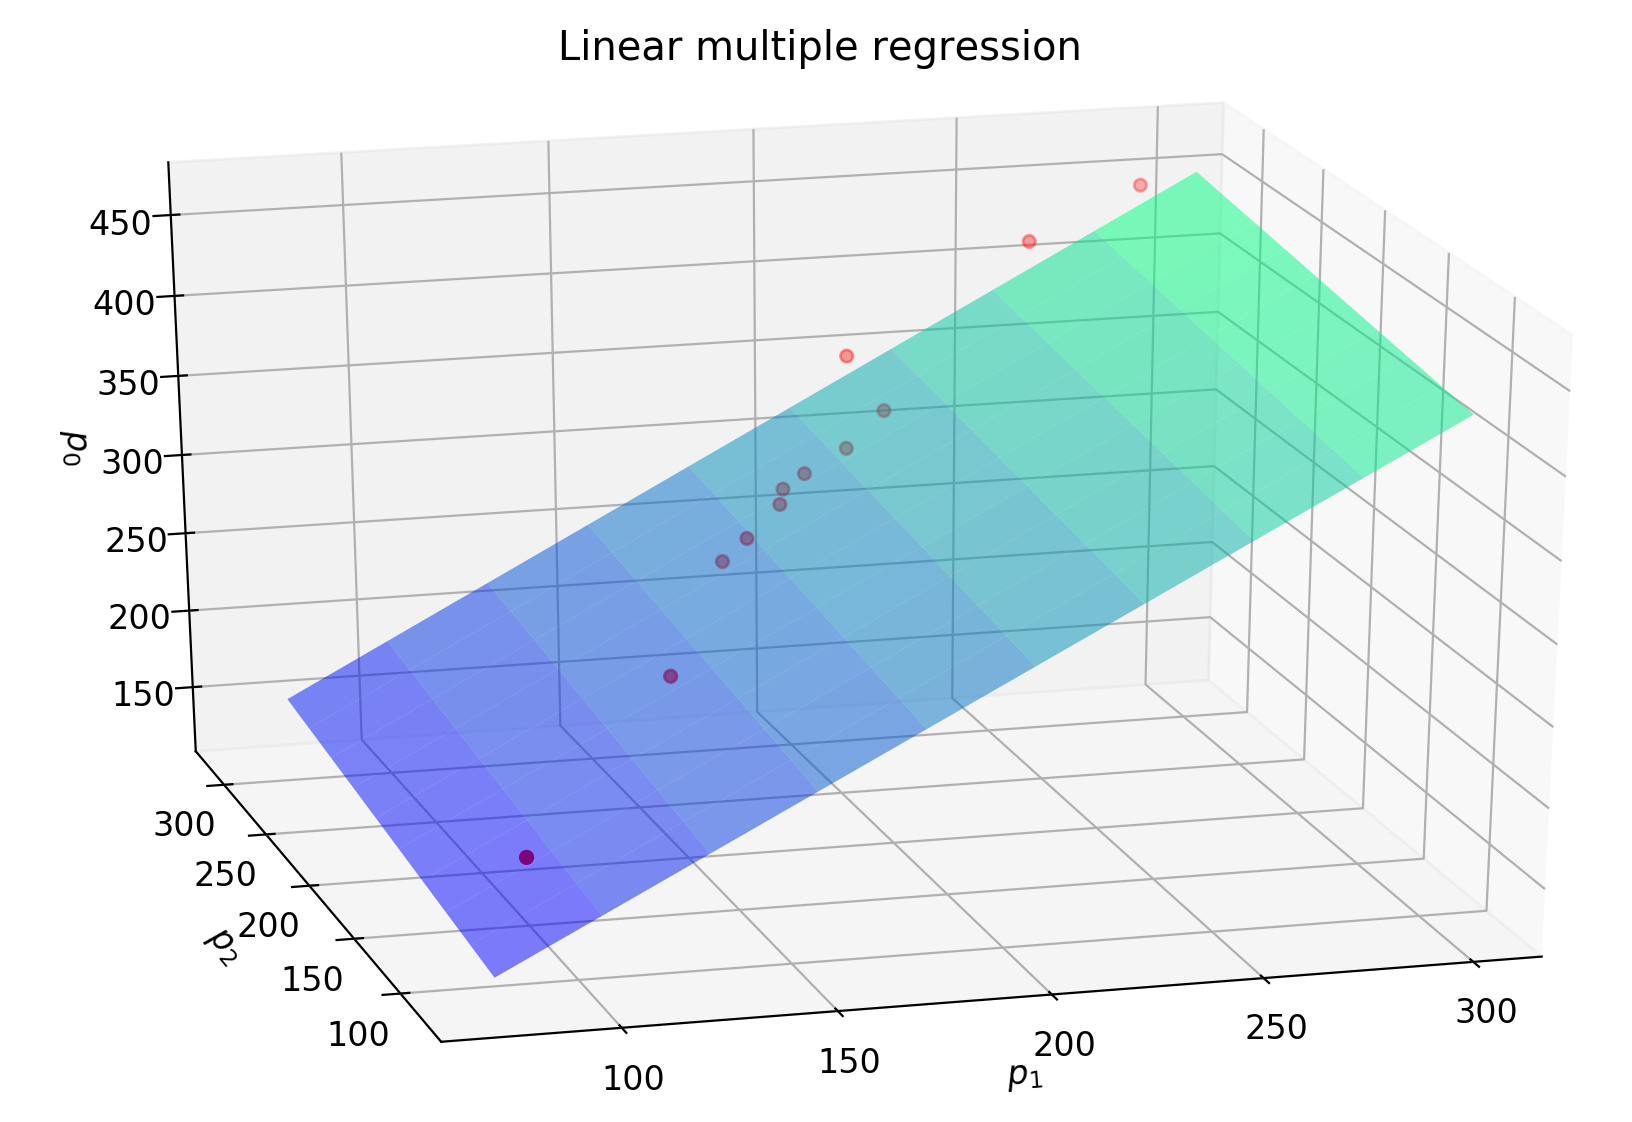
\includegraphics[width=0.65\textwidth]{Linear_Multi_Regression}
      \vspace{-1em}
    \caption{Ergebnis der linearen Mehrfachregression}
  \end{figure}
  \vspace{-1em}
  \centering

  $cond_2(A)=1787.633757$, $||Ax-b||_2=32.091986$

\end{frame}

\section{Ausblick}

\begin{frame} %%Eine Folie
  \frametitle{Alternativer Lösungsweg mit Normalengleichung} %%Folientitel
\centering

viel mehr Messwerte als Variablen $\Rightarrow$ QR-Zerlegung aufwändig
\bigskip

\underline{Normalengleichung}: $A^T Ax = A^T b$
\bigskip

\pause
\begin{tabular}{c|c|c}
  Nr. der Modifikation & $cond_2(A)$   & $cond_2(A^T A)$\\ \hline
                     0 & $\approx 820$  & $\approx 672631$\\ \hline
                     1 & $\approx 857$  & $\approx 734467$\\ \hline
                     2 & $\approx 665$  & $\approx 442594$
\end{tabular}

\pause
\bigskip

$\Rightarrow$ Ergebnisse dann evtl. viel ungenauer

\end{frame}

\begin{frame}{Quellen}
  \bibliographystyle{plain}
  \bibliography{presentation}
  \nocite{*}
\end{frame}

\end{document}
